% ****** Start of file apssamp.tex ******
%
%   This file is part of the APS files in the REVTeX 4.1 distribution.
%   Version 4.1r of REVTeX, August 2010
%
%   Copyright (c) 2009, 2010 The American Physical Society.
%
%   See the REVTeX 4 README file for restrictions and more information.
%
% TeX'ing this file requires that you have AMS-LaTeX 2.0 installed
% as well as the rest of the prerequisites for REVTeX 4.1
%
% See the REVTeX 4 README file
% It also requires running BibTeX. The commands are as follows:
%
%  1)  latex apssamp.tex
%  2)  bibtex apssamp
%  3)  latex apssamp.tex
%  4)  latex apssamp.tex
%
\documentclass[%
 reprint,
%superscriptaddress,
%groupedaddress,
%unsortedaddress,
%runinaddress,
%frontmatterverbose, 
%preprint,
%showpacs,preprintnumbers,
%nofootinbib,
%nobibnotes,
%bibnotes,
 amsmath,amssymb,
 aps,
%pra,
%prb,
%rmp,
%prstab,
%prstper,
%floatfix,
10.5pt,
]{revtex4-1}

\usepackage{graphicx}% Include figure files
\usepackage{subfigure}
\usepackage{multirow}
\usepackage{array}
\usepackage{dcolumn}% Align table columns on decimal point
\usepackage{bm}% bold math
%\usepackage{hyperref}% add hypertext capabilities
%\usepackage[mathlines]{lineno}% Enable numbering of text and display math
%\linenumbers\relax % Commence numbering lines

%\usepackage[showframe,%Uncomment any one of the following lines to test 
%%scale=0.7, marginratio={1:1, 2:3}, ignoreall,% default settings
%%text={7in,10in},centering,
%%margin=1.5in,
%%total={6.5in,8.75in}, top=1.2in, left=0.9in, includefoot,
%%height=10in,a5paper,hmargin={3cm,0.8in},
%]{geometry}

\usepackage{xeCJK}
%\setCJKmainfont[ItalicFont={KaiTi}, BoldFont={KaiTi}]{KaiTi}
\usepackage{textcomp}
\usepackage{chemfig}
\usepackage[version=4]{mhchem}
\usepackage{fontspec}
\usepackage{listings}
\usepackage{xcolor}
\usepackage{xcolor} % 定制颜色
\definecolor{mygreen}{rgb}{0,0.6,0}
\definecolor{mygray}{rgb}{0.5,0.5,0.5}
\definecolor{mymauve}{rgb}{0.58,0,0.82}
\lstset{
backgroundcolor=\color{white},      % choose the background color
basicstyle=\footnotesize\ttfamily,  % size of fonts used for the code
columns=fullflexible,
tabsize=4,
breaklines=true,               % automatic line breaking only at whitespace
captionpos=b,                  % sets the caption-position to bottom
commentstyle=\color{mygreen},  % comment style
escapeinside={\%*}{*)},        % if you want to add LaTeX within your code
keywordstyle=\color{blue},     % keyword style
stringstyle=\color{mymauve}\ttfamily,  % string literal style
frame=single,
rulesepcolor=\color{red!20!green!20!blue!20},
% identifierstyle=\color{red},
language=Mathematica,
}

\usepackage[normalem]{ulem}

\newcommand{\chuhao}{\fontsize{42pt}{44.9pt}\selectfont}    % 初号, 1.5倍行距
\newcommand{\xiaochu}{\fontsize{30pt}{40pt}\selectfont}    % 小初, 1.5倍行距
\newcommand{\yihao}{\fontsize{26pt}{36pt}\selectfont}    % 一号, 1.4倍行距
\newcommand{\erhao}{\fontsize{22pt}{28pt}\selectfont}    % 二号, 1.25倍行距
\newcommand{\xiaoer}{\fontsize{18pt}{18pt}\selectfont}    % 小二, 单倍行距
\newcommand{\sanhao}{\fontsize{16pt}{24pt}\selectfont}    % 三号, 1.5倍行距
\newcommand{\xiaosan}{\fontsize{15pt}{22pt}\selectfont}    % 小三, 1.5倍行距
\newcommand{\sihao}{\fontsize{14pt}{21pt}\selectfont}    % 四号, 1.5倍行距
\newcommand{\sihaox}{\fontsize{14pt}{28pt}\selectfont}    % 四号, 1.5倍行距
\newcommand{\banxiaosi}{\fontsize{13pt}{19.5pt}\selectfont}    % 半小四, 1.5倍行距
\newcommand{\xiaosix}{\fontsize{12pt}{24pt}\selectfont} 	% 小四, 1.5倍行距
\newcommand{\xiaosi}{\fontsize{12pt}{18pt}\selectfont}     
\newcommand{\dawuhao}{\fontsize{11pt}{11pt}\selectfont}    % 大五号, 单倍行距
\newcommand{\wuhao}{\fontsize{10.5pt}{10.5pt}\selectfont}    % 五号, 单倍行距
\newcommand{\xiaowu}{\fontsize{9pt}{9pt}\selectfont}    % 五号, 单倍行距

%\usepackage[fntef]{ctexcap}
%\CTEXsetup[number={\chinese{section}、},format={\Large\bfseries}]{section}
%\setCJKfamilyfont{fangsong}{FangSong}                      %仿宋2312 fs  
%\newcommand{\fangsong}{\CJKfamily{fangsong}}  

\usepackage{wrapfig}
\usepackage{fancyhdr}
\usepackage{fancybox}   


\usepackage{tikz}
\usepackage{circuitikz}



\newcommand{\bra}[1]{\langle #1 |}
\newcommand{\ket}[1]{| #1 \rangle}
\newcommand{\bracket}[2]{\langle #1 | #2 \rangle}
\newcommand{\bracketl}[3]{\langle #1 | #2 | #3 \rangle}
\newcommand{\func}{\mathrm \,}
\newcommand{\define}[2]{
	\begin{definition}
	\begin{description}
	\item[#1]
	#2
	\end{description}
	\end{definition}
}

\newcommand{\sch}{Schr\"odinger}
\newcommand{\grad}{\nabla}
\newcommand{\ueq}{\neq}
\newcommand{\celsius}{\ensuremath{^\circ\hspace{-0.09em}\mathrm{C}}}
\newcommand{\unit}[2]{$#1 \, \mathrm{#2}$}

\begin{document}

%\preprint{APS/123-QED}

\title{$pVT$ relation of \ce{CO2} and the phenomena of critical points }% Force line breaks with \\
%\thanks{A footnote to the article title}% give thanks

\author{Rui Li}
 %\altaffiliation[Also at ]{Physics Department, XYZ University.}%Lines break automatically or can be forced with \\
%\author{Second Author}%
%\email{3160102098@zju.edu.cn}
\affiliation{%
 Qiushi science class (chemistry)\\
 Chu Kochen Honor College
}%

%\collaboration{MUSO Collaboration}%\noaffiliation

%\author{Zong Wei Huang}
% \homepage{http://www.Second.institution.edu/~Charlie.Author}
%\affiliation{
% Second institution and/or address\\
% This line break forced% with \\
%}%
%\affiliation{
%Qiushi science class (chemistry)\\
% Chu Kochen Honor College
%}%
%\author{Delta Author}
%\affiliation{%
% Authors' institution and/or address\\
% This line break forced with \textbackslash\textbackslash
%}%

%\collaboration{CLEO Collaboration}%\noaffiliation

%\date{\today}% It is always \today, today,
             %  but any date may be explicitly specified

%\pacs{Valid PACS appear here}% PACS, the Physics and Astronomy
                             % Classification Scheme.
%\keywords{Suggested keywords}%Use showkeys class option if keyword
                              %display desired
\maketitle

\section{Introduction}
Ideal gas law can only describe gases at relatively low pressure and a high temperature. It completely neglects the interaction between gas molecules as well as the volume of them, thus it is unable to describe nor predict condensed states. Van der Waals equation, however, takes the two neglected factors into consideration, which succeeds in predicting the liquid state. 

The Van der Waals eqaution can be deduced starting from a few approximations from thermostatistical models. Sutherland potential function gives
\begin{equation}
	u(r) = 
	\begin{cases}
	-\epsilon(\frac{{r_0}}{r})^6 \quad r>{r_0}\\
	\infty \quad r\leqslant {r_0}
	\end{cases}
\end{equation}
Define $f$ as
\begin{equation}
	f = e^{-\beta u(r)}-1
\end{equation}
then virial coefficient of second grade $B_2$ can be written as
\begin{equation}
	B_2 = - \frac{N_A}{2}\int f d \overrightarrow{r}
\end{equation}
thus
\begin{equation}
	B_2  = 2\pi N_A \left[\int_0^{r_0} r^2 \, dr - \int_{r_0}^\infty f r^2 dr \right]
\end{equation}
which can be approximated as
\begin{equation}
	B_2 \sim  2\pi N_A \left[\frac{r_0^2}{3} - \frac{r_0^3 \beta u_0}{3}\right]
\end{equation}
Defining
\begin{equation}
	b = \frac{2\pi}{3}N_A r_0^3 , a = \frac{2\pi}{3}N_A^2 u_0 r_0^3
\end{equation}
$B_2$ can be rewritten as 
\begin{equation}
	B_2 = b- \frac{a}{N_A k T}
\end{equation}
thus
\begin{align*}
	pV & =  N k T \left(1+\frac{n B_2}{V}\right) \\
 	& = N k T \left(1 + \frac{n b}{V} - \frac{n a}{N_A V k T }\right) \\
 	&=  NkT\left(1+\frac{n b }{V}\right) - \frac{n^2 a}{V} 
\end{align*}
An approximation that $\frac{n b}{V}$ is comparatively small leads to
\begin{equation}
	pV = \frac{N k T}{1-\frac{nb}{V}} - \frac{n^2 a}{V}
\end{equation}
which is a equivalent form of Van der Waals equation.

At a relatively low temperature $\frac{\partial p}{\partial V} > 0$ no longer satisfies, and there exists $p_c,V_c,T_c$ such that
\begin{equation}
\begin{cases}
	\left(\frac{\partial p}{\partial V}\right)\bigg|_{V=V_c} = 0 \\
	\left(\frac{\partial^2 p}{\partial V^2}\right)\bigg|_{V=V_c} =0
\end{cases}
\end{equation}
which leads to the solution
\begin{equation}
	V_c = 3nb, T_c = \frac{8}{27 b R}, p_c = \frac{4 a}{27 b^2}
\end{equation}
which is called critical point. Around this point several phenomena can be observed.

\section{Methods and Procedures}
$pVT$ measurement apparatus - which consists of pump pressure gauge, a thermostat and a graduated tube containing \ce{CO2} - is utilized in this experiment. Pressure is accumulated gradually until it reaches 10 MPa, during the process of which several points are chosen and the height of mercury in the tube is measured. The volume per area of cross section of the tube is calculated w.r.t. the volume per area of cross section of \ce{CO2} liquid at 9.8 MPa and 20 \celsius.

\section{Results and Analysis}
\begin{table}
\centering
\caption{The fitting parameters of the Van der Waals equation}
\begin{tabular}{ccccc}\hline
$T/\celsius$ & $10^4 a$ & $b$ & $c$ & $R^2$  \\\hline
20.0 & -0.0304197 & -0.142756 & 0.944498 & 0.985071 \\
23.0 & -0.035569 & -0.116091 & 0.831901 & 0.992765 \\
25.0 & -0.0126799 & -0.0825918 & 0.74025 & 0.991335 \\
27.0 & -0.008464 & -0.0721021 & 0.705178 & 0.992875 \\
29.0 & -0.00179595 & -0.0692964 & 0.718065 & 0.994144 \\
34.2 &  0.00952114 & -0.0599663 & 0.700013 & 0.997943 \\
40.0 &  0.0136454 & -0.05091 & 0.677438 & 0.998828 \\
45.0 &  0.100063 & -0.0284707 & 0.59214 & 0.999935 \\\hline
\end{tabular}
\label{VanderWaals}
\end{table}


\begin{table*}
\centering
\caption{The raw data of the experiment, where the upper row in each box represents the pressure of the system in MPa, while the lower row the volume per kilogram of \ce{CO2}($\mathrm{m^3/kg}$).}
\resizebox{\textwidth}{!}{
\begin{tabular}{ccccccccccccccccc}\hline
 \multicolumn{17}{c}{20.0 \celsius} \\\hline
\begin{tabular}{c}
 2.42 \\
 0.0183 \\
\end{tabular}
 & 
\begin{tabular}{c}
 3.05 \\
 0.0142 \\
\end{tabular}
 & 
\begin{tabular}{c}
 4.00 \\
 0.00981 \\
\end{tabular}
 & 
\begin{tabular}{c}
 5.05 \\
 0.00676 \\
\end{tabular}
 & 
\begin{tabular}{c}
 5.55 \\
 0.00547 \\
\end{tabular}
 & 
\begin{tabular}{c}
 5.67 \\
 0.00460 \\
\end{tabular}
 & 
\begin{tabular}{c}
 5.77 \\
 0.00325 \\
\end{tabular}
 & 
\begin{tabular}{c}
 6.45 \\
 0.00166 \\
\end{tabular}
 & 
\begin{tabular}{c}
 6.72 \\
 0.00128 \\
\end{tabular}
 & 
\begin{tabular}{c}
 7.95 \\
 0.00121 \\
\end{tabular}
 & 
\begin{tabular}{c}
 9.80 \\
 0.00117 \\
\end{tabular}
 & \text{} & \text{} & \text{} & \text{} & \text{} & \text{} \\\hline
  \multicolumn{17}{c}{23.0 \celsius} \\\hline
\begin{tabular}{c}
 2.27 \\
 0.0200 \\
\end{tabular}
 & 
\begin{tabular}{c}
 2.98 \\
 0.0149 \\
\end{tabular}
 & 
\begin{tabular}{c}
 4.05 \\
 0.00983 \\
\end{tabular}
 & 
\begin{tabular}{c}
 5.11 \\
 0.00687 \\
\end{tabular}
 & 
\begin{tabular}{c}
 6.05 \\
 0.00442 \\
\end{tabular}
 & 
\begin{tabular}{c}
 6.20 \\
 0.00242 \\
\end{tabular}
 & 
\begin{tabular}{c}
 7.44 \\
 0.00136 \\
\end{tabular}
 & 
\begin{tabular}{c}
 8.45 \\
 0.00128 \\
\end{tabular}
 & 
\begin{tabular}{c}
 9.77 \\
 0.00121 \\
\end{tabular}
 & \text{} & \text{} & \text{} & \text{} & \text{} & \text{} & \text{} & \text{} \\\hline
  \multicolumn{17}{c}{25.0 \celsius} \\\hline
\begin{tabular}{c}
 2.50 \\
 0.0182 \\
\end{tabular}
 & 
\begin{tabular}{c}
 3.28 \\
 0.0133 \\
\end{tabular}
 & 
\begin{tabular}{c}
 4.00 \\
 0.0103 \\
\end{tabular}
 & 
\begin{tabular}{c}
 4.96 \\
 0.00740 \\
\end{tabular}
 & 
\begin{tabular}{c}
 6.02 \\
 0.00498 \\
\end{tabular}
 & 
\begin{tabular}{c}
 6.40 \\
 0.00317 \\
\end{tabular}
 & 
\begin{tabular}{c}
 6.80 \\
 0.00143 \\
\end{tabular}
 & 
\begin{tabular}{c}
 7.40 \\
 0.00136 \\
\end{tabular}
 & 
\begin{tabular}{c}
 8.07 \\
 0.00133 \\
\end{tabular}
 & 
\begin{tabular}{c}
 9.73 \\
 0.00125 \\
\end{tabular}
 & \text{} & \text{} & \text{} & \text{} & \text{} & \text{} & \text{} \\\hline
  \multicolumn{17}{c}{27.0 \celsius} \\\hline
\begin{tabular}{c}
 2.29 \\
 0.0203 \\
\end{tabular}
 & 
\begin{tabular}{c}
 3.08 \\
 0.0145 \\
\end{tabular}
 & 
\begin{tabular}{c}
 4.08 \\
 0.0101 \\
\end{tabular}
 & 
\begin{tabular}{c}
 4.98 \\
 0.00759 \\
\end{tabular}
 & 
\begin{tabular}{c}
 6.04 \\
 0.00517 \\
\end{tabular}
 & 
\begin{tabular}{c}
 6.48 \\
 0.00408 \\
\end{tabular}
 & 
\begin{tabular}{c}
 6.62 \\
 0.00321 \\
\end{tabular}
 & 
\begin{tabular}{c}
 6.87 \\
 0.00170 \\
\end{tabular}
 & 
\begin{tabular}{c}
 7.68 \\
 0.00140 \\
\end{tabular}
 & 
\begin{tabular}{c}
 8.48 \\
 0.00132 \\
\end{tabular}
 & 
\begin{tabular}{c}
 9.85 \\
 0.00128 \\
\end{tabular}
 & \text{} & \text{} & \text{} & \text{} & \text{} & \text{} \\\hline
  \multicolumn{17}{c}{29.0 \celsius} \\\hline
 
\begin{tabular}{c}
 2.17 \\
 0.0219 \\
\end{tabular}
 & 
\begin{tabular}{c}
 3.10 \\
 0.0146 \\
\end{tabular}
 & 
\begin{tabular}{c}
 3.99 \\
 0.0121 \\
\end{tabular}
 & 
\begin{tabular}{c}
 5.00 \\
 0.00766 \\
\end{tabular}
 & 
\begin{tabular}{c}
 6.10 \\
 0.00532 \\
\end{tabular}
 & 
\begin{tabular}{c}
 6.88 \\
 0.00362 \\
\end{tabular}
 & 
\begin{tabular}{c}
 7.10 \\
 0.00200 \\
\end{tabular}
 & 
\begin{tabular}{c}
 7.68 \\
 0.00143 \\
\end{tabular}
 & 
\begin{tabular}{c}
 8.68 \\
 0.00132 \\
\end{tabular}
 & 
\begin{tabular}{c}
 9.75 \\
 0.00132 \\
\end{tabular}
 & \text{} & \text{} & \text{} & \text{} & \text{} & \text{} & \text{} \\\hline
  \multicolumn{17}{c}{34.2 \celsius} \\\hline
\begin{tabular}{c}
 2.05 \\
 0.0235 \\
\end{tabular}
 & 
\begin{tabular}{c}
 3.01 \\
 0.0155 \\
\end{tabular}
 & 
\begin{tabular}{c}
 3.98 \\
 0.0110 \\
\end{tabular}
 & 
\begin{tabular}{c}
 4.95 \\
 0.00819 \\
\end{tabular}
 & 
\begin{tabular}{c}
 5.95 \\
 0.00604 \\
\end{tabular}
 & 
\begin{tabular}{c}
 6.90 \\
 0.00442 \\
\end{tabular}
 & 
\begin{tabular}{c}
 7.10 \\
 0.00408 \\
\end{tabular}
 & 
\begin{tabular}{c}
 7.20 \\
 0.00393 \\
\end{tabular}
 & 
\begin{tabular}{c}
 7.30 \\
 0.00377 \\
\end{tabular}
 & 
\begin{tabular}{c}
 7.40 \\
 0.00351 \\
\end{tabular}
 & 
\begin{tabular}{c}
 7.50 \\
 0.00332 \\
\end{tabular}
 & 
\begin{tabular}{c}
 7.60 \\
 0.00302 \\
\end{tabular}
 & 
\begin{tabular}{c}
 7.75 \\
 0.00279 \\
\end{tabular}
 & 
\begin{tabular}{c}
 7.78 \\
 0.00257 \\
\end{tabular}
 & 
\begin{tabular}{c}
 8.00 \\
 0.00181 \\
\end{tabular}
 & 
\begin{tabular}{c}
 8.43 \\
 0.00159 \\
\end{tabular}
 & 
\begin{tabular}{c}
 9.70 \\
 0.00143 \\
\end{tabular}
 \\\hline
  \multicolumn{17}{c}{40.0 \celsius} \\\hline
 
\begin{tabular}{c}
 2.40 \\
 0.0204 \\
\end{tabular}
 & 
\begin{tabular}{c}
 3.04 \\
 0.0159 \\
\end{tabular}
 & 
\begin{tabular}{c}
 4.00 \\
 0.0114 \\
\end{tabular}
 & 
\begin{tabular}{c}
 5.00 \\
 0.00849 \\
\end{tabular}
 & 
\begin{tabular}{c}
 5.95 \\
 0.00668 \\
\end{tabular}
 & 
\begin{tabular}{c}
 6.95 \\
 0.00494 \\
\end{tabular}
 & 
\begin{tabular}{c}
 7.42 \\
 0.00430 \\
\end{tabular}
 & 
\begin{tabular}{c}
 7.93 \\
 0.00279 \\
\end{tabular}
 & 
\begin{tabular}{c}
 8.45 \\
 0.00279 \\
\end{tabular}
 & 
\begin{tabular}{c}
 9.18 \\
 0.00189 \\
\end{tabular}
 & 
\begin{tabular}{c}
 9.78 \\
 0.00159 \\
\end{tabular}
 & \text{} & \text{} & \text{} & \text{} & \text{} & \text{} \\\hline
  \multicolumn{17}{c}{45.0 \celsius} \\\hline
 
\begin{tabular}{c}
 2.42 \\
 0.0206 \\
\end{tabular}
 & 
\begin{tabular}{c}
 3.10 \\
 0.0159 \\
\end{tabular}
 & 
\begin{tabular}{c}
 4.00 \\
 0.0116 \\
\end{tabular}
 & 
\begin{tabular}{c}
 4.98 \\
 0.00891 \\
\end{tabular}
 & 
\begin{tabular}{c}
 6.02 \\
 0.00672 \\
\end{tabular}
 & 
\begin{tabular}{c}
 7.09 \\
 0.00510 \\
\end{tabular}
 & 
\begin{tabular}{c}
 8.10 \\
 0.00385 \\
\end{tabular}
 & 
\begin{tabular}{c}
 9.68 \\
 0.00219 \\
\end{tabular}
 & \text{} & \text{} & \text{} & \text{} & \text{} & \text{} & \text{} & \text{} & \text{} \\\hline
\end{tabular}
}
\end{table*}
\begin{figure}
\centering
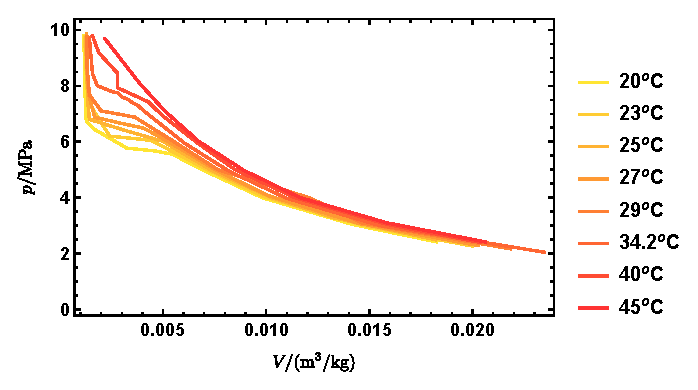
\includegraphics[width=0.48\textwidth]{figures/co2.eps}
\caption{$p-V$ line plots of \ce{CO2} at different temperature}
\label{plot}
\end{figure}
\begin{figure}
\centering
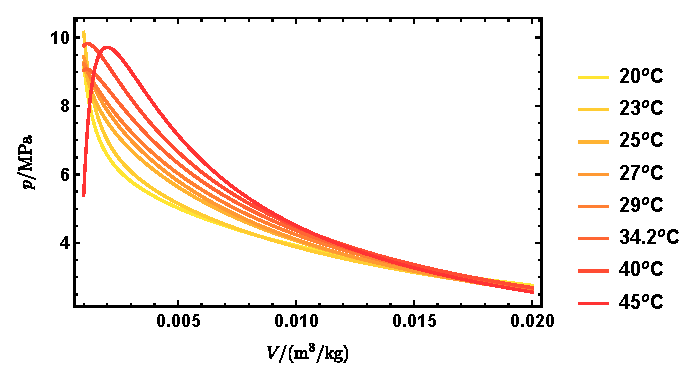
\includegraphics[width=0.48\textwidth]{figures/VanderWaalFit.eps}
\caption{$p-V$ line plots of \ce{CO2} fitted by Van der Waals equation}
\end{figure}
The $p-V$ line plots are given in Fig. \ref{plot}, with its fits by Van der Waals equation, namely
\begin{equation}
	p = \frac{c}{V-b} - \frac{a}{V^2}
\end{equation}
where $a,b,c$ are constants, and $V$ is defined as volume per kilogram of \ce{CO2}. The fitting parameters are given in Table \ref{VanderWaals}. It should be noted that only points where the \ce{CO2} only appears as one phase are considered in the fitting. Result shows that Van der Waals equation fitting fails to give a positive $b$, which might be attributed to the fluctuations of data due to deviation from equilibrium states that greatly affects the non linear fitting process, as well as the deficiency of Van der Waals equation when describing the \ce{CO2} liquid. 

The critical point is suggested as
\begin{equation}
	T_c = 307.3\, \mathrm{K},V_c = 0.00377\, \mathrm{m^3/kg},\, p_c = 7.30 \, \mathrm{MPa}
\end{equation}
while the theoretical critical point of \ce{CO2} is given as
\begin{equation}
	T_c = 304.2 \, \mathrm{K},\,  p_c = 7.38 \, \mathrm{MPa}
\end{equation}
Factors are manifold. Impurity of the \ce{CO2} as well as the deviation from equilibrium states can account for the error, while the non-uniform temperature distribution of the thermostats mainly contributes to the error in measurement of the temperature of the critical point, as is described in older reports. What makes the situation worse is that only a plastic tube with no coating materials is connected between the thermostat and the measuring device, deteriorating the circulation of the water and strengthening the heat loss. The rigidness of the tube containing \ce{CO2} should also be doubted, which may affect the measurement of volumes and a non linear effect on the $p-V$ curve.

A sudden phase transition accompanied with light scattering effect is observed, which should be attributed to very small amount of heat required for evaporation, while the fast transition leads to small radius of the liquid drops formed. Rayleigh successfully predicts the scattering light through these `particles' by regarding them as a resonance of the electromagnetic field in the particles and the light, emitting light in all directions at the same wavelength. The identical phisical properties of the liquid phase and the gas phase leads to small deviations of reflection rate between two phases, resulting in the blurred phase surface.


\section{Conclusions}
The $pVT$ curves of \ce{CO2} around its critical point is plotted. Errors in the prediction of critical points are mainly attributed to many factors, including the non uniform distribution of temperature, deviation from equilibrium states and the impurity of \ce{CO2}. Sudden phase transition is an identical phenomenon for gases near their critical points.







\end{document}
